\subsection{Результаты}
Были проведены расчеты методом HF/6-31G-CIS. Число МО 102, из них заполнено 34. Число заполненных $\pi$-орбиталей 5 (25, 29, 31, 33, 34). Число вакантных $\pi$-орбиталей 15 (35-39, 46, 55, 58, 61, 63, 70, 71, 74, 75, 83). Имеется две $n$-орбитали (30, 32), локализованные на атомах N1 и N2.
\begin{table}[H]
    \caption{Сопоставление молекулярных орбиталей, полученных разными методами}
    \begin{center}
    \label{tab:my-table}
    \resizebox{\textwidth}{!}{%
    \begin{tabular}{|c|c|c|c|}
    \hline
    \begin{tabular}[c]{@{}c@{}}Номер $\pi$-орбитали\\ из работы №8\end{tabular} & \begin{tabular}[c]{@{}c@{}}Номер $\pi$-орбитали \\ из текущей работы\end{tabular} & \begin{tabular}[c]{@{}c@{}}Номер n-орбитали\\ из работы №8\end{tabular} & \begin{tabular}[c]{@{}c@{}}Номер n-орбиталииз \\ из текущей работы\end{tabular} \\ \hline
    25 & 25 & 32 & 30 \\ \hline
    29 & 29 & 34 & 32 \\ \hline
    30 & 31 &  &  \\ \hline
    31 & -  &  &  \\ \hline
    33 & 34 &  &  \\ \hline
    35 & 35 &  &  \\ \hline
    36 & -  &  &  \\ \hline
    37 & 37 &  &  \\ \hline
    38 & 39 &  &  \\ \hline
    39 & 46 &  &  \\ \hline
    \end{tabular}%
    }
    \end{center}{}
\end{table}

Сопоставление проводилось визуально. Для МО 31, 36 не были найдены соответсвующие МО.

\begin{figure}[H]
\center
\begin{tabular}{cc}
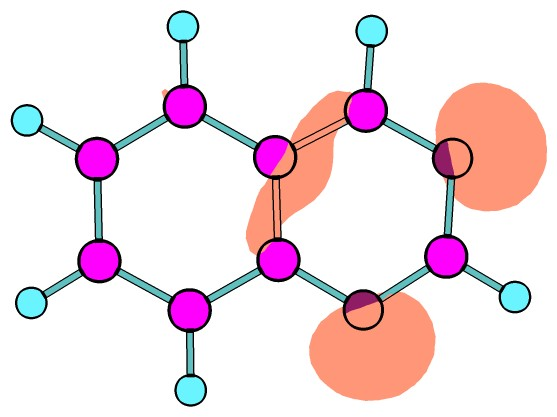
\includegraphics[scale=0.35]{fig/TDDFT-32.jpg}
&
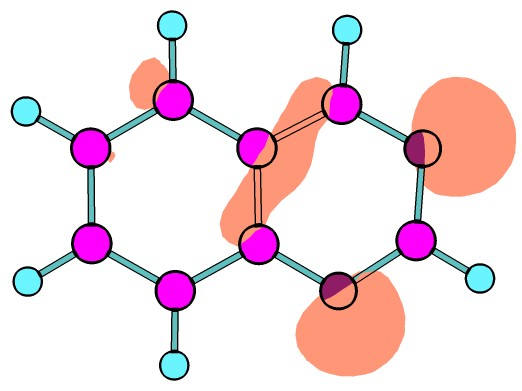
\includegraphics[scale=0.35]{fig/CIS-30.jpg}
\end{tabular}
\centering
\caption{32 (слева) и 30 (справа) МО, полученные методами TDDFT/B3LYP/3-21G и HF/6-31G-CIS соответственно.}
\end{figure}

\begin{figure}[H]
\center
\begin{tabular}{cc}
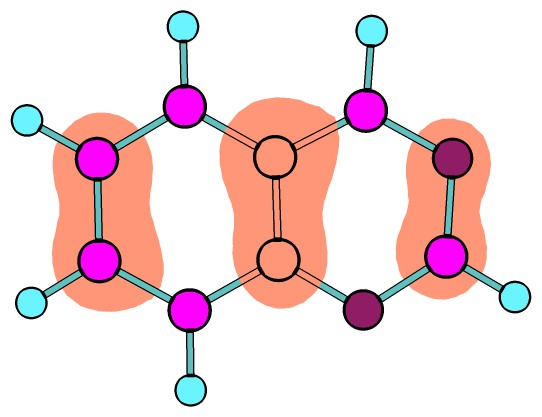
\includegraphics[scale=0.35]{fig/TDDFT-31.jpg}
&
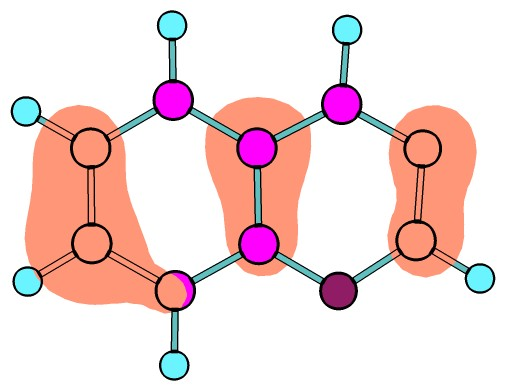
\includegraphics[scale=0.35]{fig/CIS-33.jpg}
\end{tabular}
\caption{31 (слева) и 33 (справа) МО, полученные методами TDDFT/B3LYP/3-21G и HF/6-31G-CIS соответственно. Орбитали антисимметричны.}
\end{figure}

\begin{table}[H]
    \caption{Характеристики низших возбужденных состояний}
    \label{tab:my-table}
    \begin{center}
    \resizebox{\textwidth}{!}{%
    \begin{tabular}{|c|c|c|c|c|}
    \hline
    \multirow{2}{*}{\begin{tabular}[c]{@{}c@{}}№ низшего\\ возбуждённого состояния\end{tabular}} & \multirow{2}{*}{\begin{tabular}[c]{@{}c@{}}Тип возбужденного\\ состояния\end{tabular}} & \multicolumn{2}{c|}{\begin{tabular}[c]{@{}c@{}}Энергия возбужденния\\ из основного состояния\end{tabular}} & \multirow{2}{*}{\begin{tabular}[c]{@{}c@{}}Конфигурационный\\ состав состояния\end{tabular}} \\ \cline{3-4}
     &  & эВ & см^{-1} &  \\ \hline
    1 & $\pi-\pi$ & 5.239 & 42255.4 & 34 \rightarrow 35 (-0.92117864) \\ \hline
    2 & $n-\pi$ & 5.336 & 43037.7 & 32 \rightarrow 35 (0.88995645)  \\ \hline
    3 & $\pi-\pi$ & 5.618 & 45312.2 & 33 \rightarrow 35 (0.71375864) \\ \hline
    4 & $n-\pi$ & 6.410 & 51700.1 & 32 \rightarrow 36 (0.62286527) \\ \hline
    5 & $\pi-\pi$ & 7.368 & 59426.9 & 34 \rightarrow 36 (0.52953459) \\ \hline
    6 & $n-\pi$ & 7.420 & 59846.3 & 30 \rightarrow 35 (-0.65852131) \\ \hline
    \end{tabular}
    }
    \end{center}
\end{table}

\begin{table}[H]
    \caption{Сопоставление низших возбужденных состояний, \\ полученных разными методами}
    \begin{center}
    \label{tab:my-table}
    \begin{tabular}{|c|c|}
    \hline
    \begin{tabular}[c]{@{}c@{}}Номер ВС\\ из работы №8\end{tabular} & \begin{tabular}[c]{@{}c@{}}Номер ВС\\ из текущей работы\end{tabular} \\ \hline
    1 &  -- \\ \hline
    2 &  - \\ \hline
    3 &  - \\ \hline
    4 &  1 \\ \hline
    5 &  - \\ \hline
    6 &  - \\ \hline
    \end{tabular}%
    \end{center}{}
\end{table}

Энергия возбуждения перехода 1, полученного в расчете методом HF/6-31G-CIS (5.239 эВ), оказалась по величине больше, чем в расчете методом TDDFT/B3LYP/STO-3G (5.036 эВ), но в целом не сильно отличается.
